\documentclass{article}
\usepackage{graphicx, amsmath, amssymb, mathtools, fancyhdr} % Required for inserting images
\setlength{\oddsidemargin}{0in}
\setlength{\textwidth}{6.5in}
\setlength{\topmargin}{-.55in}
\setlength{\textheight}{9in}
\pagestyle{fancy}

\graphicspath{{Images/}}

\fancyfoot{}
\fancyhead[L]{MATH 6440}
\fancyhead[R]{\thepage}

\begin{document}


\begin{center}
    {\Huge Approximation Methods HW1}
    \vspace{0.5cm}

    {\Large Michael Nameika}
    \vspace{0.5cm}

    {\large 9/14/24}
    \vspace{0.5cm}

    
\end{center}

\begin{itemize}
    \item[\textbf{1.9}] This problem derives an asymptotic approximation for the Stieltjes function, defined as
    \[S(\varepsilon) = \int_0^{\infty} \frac{e^{-t}}{1 + \varepsilon t}dt.\]
    \begin{itemize}
        \item[(a)] Find the first three terms  in the expansion of the integrand for small $\varepsilon$ and explain why this requires that $t \ll 1/\varepsilon$.
        \newline\newline
        \textit{Soln.} Notice that for $t < 1/\varepsilon$, we can expand $\frac{1}{1 + \varepsilon t} = 1 - \varepsilon t + \varepsilon^2t^2 + \cdots$. To maintain well-ordering, we make the requirement that $t \ll 1/\varepsilon$ so that 
        \begin{align*}
            \frac{e^{-t}}{1 + \varepsilon t} &\sim e^{-t}\left(1 - \varepsilon t + \varepsilon^2t^2 + \cdots\right)\\
            &= e^{-t} - \varepsilon te^{-t} + \varepsilon^2 t^2 e^{-t} + \cdots
        \end{align*}
        for $t \ll 1/\varepsilon$.
        \newline\newline
        
        \item[(b)] Split the integral into the sum of an integral over $0 < t < \delta $ and one over $\delta < t < \infty$, where $1 \ll \delta \ll 1/\varepsilon$. Explain why the second integral is bounded by $e^{-\delta}$, and use your expansion in part (a) to find an approximation for the first integral. From this derive the following approximation:
        \[S(\varepsilon) \sim 1 - \varepsilon + 2\varepsilon^2 + \cdots.\]
        \textit{Soln.} Let $ 1 \ll \delta \ll 1/\varepsilon$ and split the integral over $0 < t < \delta$ and $\delta < t <\infty$:
        \begin{align*}
            \int_0^{\infty} \frac{e^{-t}}{1 + \varepsilon t}dt &= \int_0^{\delta} \frac{e^{-t}}{1 + \varepsilon t}dt + \int_{\delta}^{\infty} \frac{e^{-t}}{1 + \varepsilon t}dt.
        \end{align*}
        For the first integral on the RHS, we can use our expansion in part (a), so that
        \[\int_0^{\delta} \frac{e^{-t}}{1 + \varepsilon t}dt \sim \int_0^{\delta} \left(e^{-t} - \varepsilon t e^{-t} + \varepsilon^2t^2e^{-t}\right)dt.\]
        Evaluating the integral of $t^2e^{-t}$, set $u = t^2$ so that $du = 2t$ and $dv = e^{-t}dt$ so that $v = -e^{-t}$ and by integration by parts, we find
        \begin{align*}
            \int_0^{\delta} t^2e^{-t}dt &= \left[-t^2e^{-t}\right]\big|_0^{\delta} + 2\int_0^{\delta}te^{-t}dt \\
            &= -\delta^2e^{-\delta} + 2\int_0^{\delta} te^{-t}dt.
        \end{align*}
        For the remaining integral, set $u = t$ so that $du = dt$ and set $dv = e^{-t}dt$ so $v = -e^{-t}$ and by integration by parts we have
        \begin{align*}
            \int_0^{\delta} te^{-t} dt &= \left[-te^{-t}\right]\big|_0^{\delta} + \int_0^{\delta}e^{-t}dt\\
            &= -\delta e^{-\delta} + 1 - e^{-\delta}.
        \end{align*}
        Putting this together, we find
        \begin{align*}
            \int_0^{\delta} \left(e^{-t} - \varepsilon te^{-t} + \varepsilon^2 t^2e^{-t}\right)dt &= 1 - e^{-\delta} - \varepsilon\left(-\delta e^{-\delta} + 1 - e^{-\delta}\right) + 2\varepsilon^2\left(-\delta^2e^{-\delta} - 2\delta e^{-\delta} - e^{-\delta} + 1\right).\\
            &= (1 - e^{-\delta})(1 - \varepsilon + 2\varepsilon^2 + \cdots) + e^{-\delta}(-\varepsilon \delta - 2\varepsilon^2\delta^2 - 4\delta\varepsilon^2 + \cdots)
        \end{align*}
        let $\alpha = \varepsilon\delta$ so that the above expression becomes
        \begin{align*}
            (1 - e^{-\alpha/\varepsilon})(1 - \varepsilon + 2\varepsilon^2 + \cdots) + e^{-\alpha/\varepsilon}(- \alpha - 2\alpha^2 + \frac{\alpha}{\delta}+ \cdots) &= (1 - e^{-\alpha/\varepsilon})(1 - \varepsilon + 2\varepsilon^2 + \cdots) + e^{-\alpha/\varepsilon}\mathcal{O}(\alpha)\\
            &\sim (1 - e^{-\alpha/\varepsilon})(1 - \varepsilon + 2\varepsilon^2 + \cdots) 
        \end{align*}
        since $e^{-\alpha/\varepsilon} = o(\varepsilon^{n})$ for all $n \in \mathbb{N}$, as we now show. Let $t = 1/\varepsilon$ so that $t \to \infty$ as $\varepsilon \to 0^+$, so that
        \begin{align*}
            \lim_{\varepsilon \to 0^+}\frac{e^{-\alpha/\varepsilon}}{\varepsilon^n} &= \lim_{t \to \infty}\frac{t^n}{e^{\alpha t}}
        \end{align*}
        and after $n$ applications of $L'Hopital's$ rule, we find
        \begin{align*}
            \lim_{t \to \infty}\frac{t^n}{e^{\alpha t}} &= \lim_{t \to \infty}\frac{n!}{\alpha^ne^{\alpha t}}\\
            &= 0
        \end{align*}
        so that $e^{-\alpha/\varepsilon} = o(\varepsilon^n)$ as $\varepsilon \to 0^+$. Using this, we find
        \begin{align*}
            1 - \varepsilon + 2\varepsilon^2 + \cdots - e^{-\alpha/\varepsilon}(1 - \varepsilon + 2\varepsilon^2 + \cdots) &\sim 1 - \varepsilon + 2\varepsilon^2 + \cdots.
        \end{align*}
        For the integral over $(\delta, \infty)$, notice
        \begin{align*}
            \int_{\delta}^{\infty}\frac{e^{-t}}{1 + \varepsilon t}dt &\leq \int_{\delta}^{\infty} e^{-t}dt\\
            &= e^{-\delta}\\
            &= e^{-\alpha/\varepsilon}\\
            \implies \int_{\delta}^{\infty} \frac{e^{-t}}{1 + \varepsilon t}dt &= o(\varepsilon^n).
        \end{align*}
        Putting it together, we have
        \begin{align*}
            \int_0^{\infty} \frac{e^{-t}}{1 + \varepsilon t}dt &\sim 1 - \varepsilon + 2\varepsilon^2 + \cdots + e^{-\alpha/\varepsilon}\\
            &\sim 1 - \varepsilon + 2\varepsilon^2 + \cdots
        \end{align*}
        as desired.
        
    \end{itemize}   

    \pagebreak


    \item[\textbf{1.16}] This problem derives asymptotic approximations for the complete elliptic integral, defined as
    \[K(x) = \int_0^{\pi/2}\frac{ds}{\sqrt{1 - x\sin^2(s)}}.\]
    It is assumed that $0 < x < 1$.
    \begin{itemize}
        \item[(a)] Show that, for $x$ close to zero, $K \sim \frac{\pi}{2}(1 + \frac{1}{4}x).$
        \newline\newline
        \textit{Proof:} By the binomial expansion, we have (near $x = 0$)
        \begin{align*}
            (1 - ax)^{-1/2} &= \sum_{k = 0}^{\infty} \begin{pmatrix}
                -1/2\\
                k
            \end{pmatrix}(-ax)^k\\
            &= 1 + \frac{1}{2}ax + \cdots.
        \end{align*}
        Using this, our integrand has the expansion 
        \[\frac{1}{\sqrt{1 - x\sin^2(s)}} \sim 1 + \frac{1}{2}x\sin^2(s) + \cdots.\]
        Then our integral becomes
        \begin{align*}
            \int_0^{\pi/2}\frac{ds}{\sqrt{1 - x\sin^2(s)}} &\sim \int_0^{\pi/2} \left(1 + \frac{x}{2}\sin^2(s)\right)ds\\
            &= \pi/2 + \frac{x}{4}\left(\frac{\pi}{2} - \left[\frac{1}{2}\sin(2s)\right]\bigg|_0^{\pi/2}\right)\\
            &= \frac{\pi}{2} + \frac{x}{4}\left(\frac{\pi}{2}\right)\\
            &= \frac{\pi}{2}\left(1 + \frac{1}{4}x\right)
        \end{align*}
        so that 
        \[K(x) \sim \frac{\pi}{2}\left(1 + \frac{1}{4}x\right)\]
        as $x \to 0$, as desired.
        \newline\newline
        
        

        \item[(b)] Show that, for $x$ close to one, $K \sim -\frac{1}{2}\ln(1 - x).$
        \newline\newline
        \textit{Proof:} Let $\varepsilon = 1 - x$ and $0 < \delta = \delta(\varepsilon) \ll 1$. We will inspect the integral 
        \[\int_0^{\pi/2 - \delta} \frac{ds}{\sqrt{1 - x\sin^2(s)}}\]
        as $\delta \to 0$ since the integrand is unintegrable near $s = \pi/2$ when $x = 1$. Begin by expanding the integrand $\frac{1}{\sqrt{1 - x\sin^2(s)}}$ near $x = 1$. Evaluating the first couple terms of the Taylor series, we have
        \begin{align*}
            \frac{1}{\sqrt{1 - x\sin^2(s)}} &= \sum_{n = 0}^{\infty} a_nx^n
        \end{align*}
        and recall that $a_0 = \frac{1}{\sqrt{1 - x\sin^2(s)}}\bigg|_{x = 1} = \sec(s)$, $a_1 = \frac{d}{dx}\frac{1}{\sqrt{1 - x\sin^2(s)}}\bigg|_{x = 1} = \frac{-\sin^2(s)}{2(1 - x\sin^2(s))^{3/2}}\bigg|_{x = 1} = -\frac{1}{2}\sec(s)\tan^2(s)$. Then the first two terms in our expansion becomes
        \begin{align*}
            \frac{1}{\sqrt{1 - x\sin^2(s)}} &= \sec(s) - \frac{1-x}{2}\sec(s)\tan^2(s) + \cdots\\
            \implies \int_0^{\pi/2 - \delta}\frac{ds}{\sqrt{1 - x\sin^2(s)}} &\sim \int_0^{\pi/2-\delta}\sec(s)\left(1 - \frac{\varepsilon}{2}\tan^2(s)\right)ds\\
            &= \int_0^{\pi/2 - \delta}\sec(s)ds - \frac{\varepsilon}{2}\int_0^{\pi/2 - \delta} \sec(s)\tan^2(s)ds.
        \end{align*}
        The first integral evaluates to 
        \begin{align*}
            \int_0^{\pi/2 - \delta}\sec(s)ds &= \left[\ln(\sec(s) + \tan(s))\right]\bigg|_0^{\pi/2 - \delta}\\
            &= \ln\left(\frac{1 + \sin(\pi/2 - \delta)}{\cos(\pi/2 - \delta)}\right)\\
            &= \ln\left(\frac{1 + \cos(\delta)}{\sin(\delta)}\right).
        \end{align*}
        And for $\delta \ll 1$, $\cos(\delta) \sim 1 - \delta^2/2 + \cdots$ and $\sin(\delta) \sim \delta - \delta^3/3! + \cdots$, hence $\frac{1 + \cos(\delta)}{\sin(\delta)} \sim \frac{2}{\delta}\left(\frac{1}{1 - \delta^2/6 + \cdots}\right)$ so that
        \begin{align*}
            \ln\left(\frac{1 + \cos(\delta)}{\sin(\delta)}\right) &\sim \ln(2) - \ln(\delta) + \ln(1 + \delta^2/6 + \cdots)\\
            &\sim \ln(2) - \ln(\delta) - \delta^2/6 + \cdots
        \end{align*}
        Now, evaluating the second integral, we have
        \begin{align*}
            \int_0^{\pi/2 - \delta} \sec(s)\tan^2(s)ds &= \int_0^{\pi/2 - \delta} \sec(s)(\sec^2(s) - 1)ds\\
            &= \int_0^{\pi/2 - \delta} \sec^3(s)ds - \int_0^{\pi/2 - \delta}\sec(s)ds.
        \end{align*}
        Now to evaluate ${\displaystyle \int_0^{\pi/2-\delta} \sec^3(s)ds }$, let $u = \sec(s)$ so that $ds = \sec(s)\tan(s)ds$ and $dv = \sec^2(s)ds$ so that $v = \tan(s)$. Then by integration by parts, we have
        \begin{align*}
            \int_0^{\pi/2 - \delta} \sec^3(s)ds &= \left[\sec(s)\tan(s)\right]\bigg|_0^{\pi/2 - \delta} - \int_0^{\pi/2 - \delta}\sec(s)\tan^2(s)ds.
        \end{align*}
        Thus,
        \begin{align*}
            \int_0^{\pi/2 - \delta} \sec(s)\tan^2(s)ds &= \left[\sec(s)\tan(s)\right]\bigg|_0^{\pi/2 - \delta} - \left[\ln(\sec(s) + \tan(s)\right]\bigg|_0^{\pi/2 - \delta} - \int_0^{\pi/2 - \delta}\sec(s)\tan^2(s)ds\\
            \implies 2\int_0^{\pi/2 - \delta} \sec(s)\tan^2(s)ds &= \left[\sec(s)\tan(s) - \ln(\sec(s) + \tan(s))\right]\bigg|_0^{\pi/2 - \delta}\\
            \implies \int_0^{\pi/2 - \delta} \sec(s)\tan^2(s)ds &= \frac{1}{2}\left[\sec(s)\tan(s) - \ln(\sec(s) + \tan(s))\right]\bigg|_0^{\pi/2 - \delta}\\
            &= \frac{1}{2}\left(\sec(\pi/2 - \delta)\tan(\pi/2 - \delta) - \ln(\sec(\pi/2 - \delta) + \tan(\pi/2 - \delta)) - 0 + \ln(1)\right)\\
            &= \frac{1}{2}\left(\frac{\cos(\delta)}{\sin^2(\delta)} - \ln\left(\frac{1 + \cos(\delta)}{\sin(\delta)}\right)\right).
        \end{align*}
        And $\cos(\delta) \sim 1 - \delta^2/2 + \cdots$, $\sin(\delta) \sim \delta - \delta^3/3! + \cdots$, $\sin^2(\delta) \sim \delta^2 - \delta^4/3 + \cdots$, hence
        \begin{align*}
            \frac{\cos(\delta)}{\sin^2(\delta)} &\sim \frac{1 - \delta^2/2 + \cdots}{\delta^2 - \delta^4/3 + \cdots}\\
            &= \frac{1}{\delta^2}\left(\frac{1 - \delta^2/2 + \cdots}{1 - \delta^2/3 + \cdots}\right)\\
            &\sim \frac{1}{\delta^2}(1 - \delta^2/2 + \cdots)(1 + \delta^2/3 + \cdots)\\
            &\sim \frac{1}{\delta^2}(1 - \delta^2/6 + \cdots)\\
            &\sim \frac{1}{\delta^2} - \frac{1}{6} + \mathcal{O}(\delta).
        \end{align*}
        
        Now note that $\delta^n = o(\log(\delta))$ since $\lim_{\delta \to 0^+} \frac{\delta^n}{\log(\delta)} = \lim_{\delta \to 0^+} n\delta^n = 0$. Note further that $c \in \mathbb{R}$ is $o(\log(\delta))$ since $\lim_{\delta \to 0^+} \frac{c}{\log(\delta)} = 0$. 
        Putting it together, we have
        \begin{align*}
            \int_0^{\pi/2 - \delta} \frac{ds}{\sqrt{1 - x\sin^2(s)}} &\sim \ln(2) - \ln(\delta) - \frac{\varepsilon}{4}\left(\frac{1}{\delta^2} - \frac{1}{6} - \frac{1}{2}\ln(2) + \frac{1}{2}\ln(\delta)\right)\\
        \end{align*}
        Applying dominated balance, we want $\frac{\varepsilon}{\delta^2}$ to have lower order than $\log(\varepsilon)$ since . Setting $\delta = \sqrt{\varepsilon}$ will achieve this. Thus, 
        \begin{align*}
            \int_0^{\pi/2 - \sqrt{\varepsilon}} \frac{ds}{\sqrt{1 - x\sin^2(s)}} &\sim \ln(2) - \frac{1}{4} -\frac{1}{2}\ln(\varepsilon) + \frac{\varepsilon}{48} - \frac{\varepsilon}{8}\ln(\varepsilon) + \frac{\varepsilon}{8}\\
            &= \ln(2) - \frac{1}{4} - \frac{1}{2}\ln(1 - x) + \frac{(1-x)}{48} - \frac{1 - x}{8}\ln(1-x) + \frac{1 - x}{8}.
        \end{align*}
        And since $\varepsilon^n = o(\ln(\varepsilon))$ as $\varepsilon \to 0^+$ for all $n \in \mathbb{N}$ we have, to leading order,
        \begin{align*}
            \int_0^{\pi/2 - \sqrt{\varepsilon}} \frac{ds}{\sqrt{1 - x\sin^2(s)}} &\sim -\frac{1}{2}\ln(1-x) 
        \end{align*}
        since $(1 - x)\log(1 - x) = o(\log(1-x))$ by 
        \begin{align*}
            \lim_{x \to 1^-} \frac{(1-x)\log(1-x)}{\log(1-x)} &= \lim_{x \to 1^-} (1-x) = 0
        \end{align*}
        as desired.
        \newline\newline
 
        \item[(c)] Show that, for $x$ close to one, 
        \[K \sim -\frac{1}{2}\left[1 + \frac{1}{4}(1 - x)\right]\ln(1 - x).\]
        \textit{Proof:} Note that a constant $c\in \mathbb{R}$ is not $o(\log(\delta))$, so we need to cancel out the constant terms that we found in part (b). To do so, instead of setting $\delta = \sqrt{\varepsilon}$, set $\delta = c\sqrt{\varepsilon}$ where $c \in \mathbb{R}$. From part (b), we find
        \begin{align*}
            \int_0^{\pi/2 - \delta} \frac{ds}{\sqrt{1 - x\sin^2(s)}} &\sim \ln(2) - \ln(\delta) - \frac{\varepsilon}{4}\left(\frac{1}{\delta^2} - \frac{1}{6} - \ln(2) + \ln(\delta)\right)\\
            &\sim \ln(2) - \frac{1}{2}\ln(\varepsilon) - \ln(c) -\frac{1}{4c^2} - \frac{\varepsilon}{8}\ln(\varepsilon)
        \end{align*}
        we require $c$ to be such that the constant terms in the above equations cancel out. That is, we require
        \begin{align*}
            \ln(2) - \frac{1}{4c^2} - \log(c) &= 0\\
            \implies 4c^2\log(c) - 4c^2 \log(2) + 1 &= 0.
        \end{align*}
        Let $f(c) = 4c^2\log(c) - 4c^2\log(2) + 1$. Notice $f$ is continuous for $c > 0$ and $\lim_{c \to 0^+} f(c) = 1$. Now notice $f(1) = 1 - 2\ln(2) < 0$. Thus by the intermediate value theorem, there exists at least one root satisfying $0 < c < 1$. Let $c$ satisfy $f(c) = 0$. Then we have
        \begin{align*}
            \int_0^{\pi/2 - c\sqrt{\varepsilon}}\frac{ds}{\sqrt{1 - x\sin^2(s)}} &\sim -\frac{1}{2}\ln(\varepsilon) - \frac{\varepsilon}{8}\ln(\varepsilon)\\
            &= -\frac{1}{2}\left(1 + \frac{\varepsilon}{4}\right)\ln(\varepsilon)\\
            &= -\frac{1}{2}\left(1 + \frac{1-x}{4}\right)\ln(1-x)
        \end{align*}
        as desired.
    \end{itemize}

    \pagebreak

    \item[\textbf{1.18}] Find a two-term asymptotic expansion, for small $\varepsilon$, of each solution $x$ of the following equations:
    \begin{itemize}
        \item[(f)] $\varepsilon^2x^3 - x + \varepsilon = 0$
        \newline\newline
        \textit{Soln:} Assume $x(\varepsilon) = x_0 + \varepsilon^{\alpha} x_1 + \varepsilon^{2\alpha} x_2 + \varepsilon^{3\alpha} x_3 + \varepsilon^{4\alpha}x_4 + \cdots$. Then
        \begin{align*}
            x^3 &= (x_0 + \varepsilon^{\alpha} x_1 + \varepsilon^{2\alpha} x_2 + \varepsilon^{3\alpha} x_3 + \varepsilon^{4\alpha} x_4 + \cdots)^3\\
            &= x_0^3 + 3\varepsilon^{\alpha} x_0^2x_1 + 3\varepsilon^{2\alpha}x_0x_1^2 + 3\varepsilon^{2\alpha}x_0^2x_2 \varepsilon^{3\alpha}x_1^3 + 6\varepsilon^{3\alpha}x_0x_1x_2 + \cdots \\
            \implies \varepsilon^{2}x(\varepsilon)^3 &= \varepsilon^2x_0^3 + 3\varepsilon^{2 + \alpha}x_0^2x_1 + 3\varepsilon^{2 + 2\alpha}x_0x_1^2 + 3\varepsilon^{2 + 2\alpha}x_0^2x_2 + \cdots.
        \end{align*}
        Putting this expansion into our algebraic equation, we have
        \begin{align*}
            &\varepsilon^2x_0^3 + 3\varepsilon^{2 + \alpha}x_0^2x_1 + 3\varepsilon^{2 + 2\alpha}x_0x_1^2 + 3\varepsilon^{2 + 2\alpha}x_0^2x_2 + \\
            & + \varepsilon^{2 + 3\alpha} x_1^3 + 6\varepsilon^{2 + 3\alpha}x_0x_1x_2 + \cdots - x_0 - \varepsilon^{\alpha} x_1 - \varepsilon^{2\alpha} x_2 - \varepsilon^{3\alpha}x_3 - \varepsilon^{4\alpha}x_4 - \varepsilon^{5\alpha}x_5 + \cdots + \varepsilon = 0.
        \end{align*}
        Matching orders, we have 
        \begin{align*}
            &\mathcal{O}(1): -x_0 = 0 \implies x_0 = 0
        \end{align*}
        we must balance the $\varepsilon$ term, and lowest order term with respect to $\alpha$ is $\varepsilon^{\alpha}$, so we require $\alpha = 1$ and we find
        \begin{align*}
            &\mathcal{O}(\varepsilon): 1 - x_1 = 0 \implies x_1 = 1\\
            &\mathcal{O}(\varepsilon^2): -x_2 + x_0^3 = -x_2 = 0 \implies x_2 = 0\\
            &\mathcal{O}(\varepsilon^3): -x_3 + 3x_0^2x_1 = -x_3 \implies x_3 = 0\\
            &\mathcal{O}(\varepsilon^4): 3x_0x_1^2 + 3x_0^2x_2 - x_4 = -x_4 = 0 \implies x_4 = 0\\
            &\mathcal{O}(\varepsilon^5): 6x_0x_1x_2 + x_1^3 - x_5 = 1 - x_5 = 0 \implies x_5 = 1.
        \end{align*}
        Hence we have
        \[x \sim \varepsilon + \varepsilon^5.\]
        Since our algebraic equation is cubic, we expect to find two other roots to the equation. To find these other roots, assume $x(\varepsilon) = \varepsilon^{\gamma}(x_0 + \varepsilon^{\alpha}x_1 + \varepsilon^{2\alpha}x_2 + \cdots)$. Then our algebraic equation becomes
        \begin{align*}
            \varepsilon^{2 + 3\gamma}(x_0 + \varepsilon^{\alpha}x_1 + \varepsilon^{2\alpha}x_2 + \cdots)^3 - \varepsilon^{\gamma}(x_0 + \varepsilon^{\alpha}x_1 + \varepsilon^{2\alpha}x_2 + \cdots) + \varepsilon &= 0\\
            \varepsilon^{2 + 3\gamma}(x_0^3 + 3\varepsilon^{\alpha}x_0^2x_1 + 3\varepsilon^{2\alpha}x_0x_1^2 + \cdots) - \varepsilon^{\gamma}(x_0 + \varepsilon^{\alpha}x_1 + \varepsilon^{2\alpha}x_2 + \cdots) + \varepsilon &= 0.
        \end{align*}
        We now seek to balance terms. Let $(1)$ denote $\varepsilon^{2 + 3\gamma}(x_0^3 + 3\varepsilon^{\alpha}x_0^2x_1 + 3\varepsilon^{2\alpha}x_0x_1^2 + \cdots)$, $(2)$ denote $-\varepsilon^{\gamma}(x_0 + \varepsilon^{\alpha}x_1 + \varepsilon^{2\alpha}x_2 + \cdots)$ and $(3)$ denote $\varepsilon$. First assume that $(1)$ balances with $(3)$ and $(2)$ is of higher order. Then we have $$2 + 3\gamma = 1 \implies \gamma = -1/3.$$ But then $(2) = \mathcal{O}(\varepsilon^{-1/3})$, contrary to our assumption. Now assume $(1)$ balances with $(2)$. Then $$2 + 3\gamma = \gamma \implies \gamma = -1$$ and $(3)$ is of higher order, consistent with our assumption. Rewriting our expansion (after multiplying by $\varepsilon$), we have
        \[x_0^3 + 3\varepsilon^{\alpha}x_0^2x_1 + 3\varepsilon^{2\alpha}x_0x_1^2 + \cdots - x_0 - \varepsilon^{\alpha}x_1 - \varepsilon^{2\alpha} + \cdots + \varepsilon^2 = 0.\]
        For $\mathcal{O}(1)$, we have $x_0^3 - x_0 = 0$ giving $x_0(x_0^2 - 1) = 0$ giving 
        \[x_0 = \pm 1, 0.\]
        The case where $x_0 = 0$ gives the root near zero, so we focus on $x_0 = \pm 1$. First suppose $x_0 = 1$. We now have two cases:
        \newline\newline
        Case 1: $\varepsilon^{\alpha}$ is of lower order than $\varepsilon^2$. Then our $\mathcal{O}(\varepsilon^{\alpha})$ terms give
        \begin{align*}
            3x_0^2x_1 - x_1 &= 0\\
            \implies x_1 &= 0.
        \end{align*}
        Further, to balance the $\mathcal{O}(\varepsilon^2)$, we require $\alpha = 1$, so that our $\mathcal{O}(\varepsilon^2)$ terms give
        \begin{align*}
            3x_0x_1^2 + 3x_2x_0^2 - x_2 + 1 &= 0\\
            \implies 3x_1^2 + 3x_2 - x_2 + 1 &= 0\\
            \implies 2x_2 &= -1\\
            \implies x_2 &= -\frac{1}{2}.
        \end{align*}
        Case 2: $\varepsilon^{\alpha}$ is of the same order of $\varepsilon^2$, giving $\alpha = 2$ and so the $\mathcal{O}(\varepsilon^2)$ terms give
        \begin{align*}
            3x_0^2x_1 - x_1 + 1 &= 0\\
            \implies 3x_1 - x_1 + 1 &= 0\\
            \implies 2x_1 &= -1\\
            \implies x_1 &= -\frac{1}{2}.
        \end{align*}
        In either case, we have
        \[x \sim \frac{1}{\varepsilon} - \frac{\varepsilon}{2}.\]
        Now suppose $x_0 = -1$. Similar to above, consider the following cases:
        \newline\newline
        Case 1: $\varepsilon^{\alpha}$ is of lower order than $\varepsilon^2$. Then our $\mathcal{O}(\varepsilon^{\alpha})$ terms, we have
        \begin{align*}
            3x_0^2x_1 - x_1 &= 0\\
            \implies x_1 &= 0.
        \end{align*}
        To balance the $\varepsilon^2$ term, we have $\alpha = 1$ and so our $\mathcal{O}(\varepsilon^2)$ terms give
        \begin{align*}
            3x_0x_1^2 + 3x_2x_0^2 - x_2 + 1 &= 0\\
            \implies 3x_2 - x_2 + 1 &= 0\\
            \implies 2x_2 &= -1\\
            \implies x_2 &= -\frac{1}{2}.
        \end{align*}
        Case 2: $\varepsilon^{\alpha}$ is of the same order of $\varepsilon^2$. Then $\alpha = 2$ and our $\mathcal{O}(\varepsilon^2)$ terms give
        \begin{align*}
            3x_0^2x_1 - x_1 + 1 &= 0\\
            \implies 3x_1 - x_1 + 1 &= 0\\
            \implies 2x_1 &= -1\\
            \implies x_1 &= -\frac{1}{2}.
        \end{align*}
        So in either case, we have 
        \[x \sim -\frac{1}{\varepsilon} - \frac{\varepsilon}{2}.\]
        Thus, our two-term expansions for the three roots of this equation are
        \begin{align*}
            x^{(0)} &\sim \varepsilon + \varepsilon^5\\
            x^{(1)} &\sim \frac{1}{\varepsilon} - \frac{\varepsilon}{2}\\
            x^{(2)} &\sim -\frac{1}{\varepsilon} - \frac{\varepsilon}{2}.
        \end{align*}
        
        
        \item[(h)] $x^2 + \varepsilon\sqrt{2 + x} = \cos(\varepsilon)$
        \newline\newline
        \textit{Soln:} Note that for $\varepsilon = 0$, we have $x^2 = 1 \implies x = \pm 1$ so that we have two solutions near 0, and within the radius of convergence of the binomial expansion of $\sqrt{2 + x}$. Thus, we begin by expanding $\sqrt{2 + x}:$
        \begin{align*}
            \sqrt{2 + x} &= \sum_{k = 0}^{\infty} \begin{pmatrix}
                1/2\\
                k
            \end{pmatrix}2^{1/2-k}x^k\\
            &= \sqrt{2} + \frac{1}{2\sqrt{2}}x + \frac{1}{8\sqrt{8}}x^2 + \cdots.
        \end{align*}
        Now assume
        \[x(\varepsilon) = x_0 + \varepsilon x_1 + \varepsilon^2x_2 + \cdots.\]
        Putting this expansion into our binomial expansion yields
        \[\sqrt{2 + x(\varepsilon)} = \sqrt{2} + \frac{1}{2\sqrt{2}}(x_0 + \varepsilon x_1 + \cdots) + \frac{1}{8\sqrt{8}}(x_0 + \varepsilon x_1 + \cdots)^2 + \cdots\]
        Expanding $\cos(\varepsilon)$ near $\varepsilon = 0$ gives
        \[\cos(\varepsilon) = 1 - \frac{\varepsilon^2}{2} + \cdots\]
        and putting this all into our original algebraic equation yields
        \begin{align*}
            &x(\varepsilon)^2 + \varepsilon\sqrt{2 + x(\varepsilon)} - \cos(\varepsilon) = \\
            &=x_0^2 + 2\varepsilon x_0x_1 + \varepsilon^2 x_1^2 + 2\varepsilon^2x_0x_2 + \cdots + \varepsilon\left(\sqrt{2} + \frac{1}{2\sqrt{2}}x_0 + \frac{1}{8\sqrt{8}}x_0^2 + \mathcal{O}(\varepsilon)\right) - 1 + \frac{\varepsilon^2}{2} + \cdots = 0\\
            &= x_0^2 + 2\varepsilon x_0x_1 + \varepsilon^2 x_1^2 + 2\varepsilon^2 x_0x_2 + \cdots + \varepsilon\sqrt{2 + x_0} - 1 + \mathcal{O}(\varepsilon^2) = 0
        \end{align*}
        where we used that to leading order, we recover the binomial expansion for $\sqrt{2 + x_0}$. Collecting terms order-by-order gives
        \begin{align*}
            &\mathcal{O}(1): x_0^2 - 1 = 0 \implies x_0 = \pm 1.
        \end{align*}
        First consider the case $x_0 = 1$. Then
        \begin{align*}
            &\mathcal{O}(\varepsilon): 2x_0x_1 + \sqrt{2 + x_0} = 2x_1 + \sqrt{3} = 0 \implies x_1 = -\frac{\sqrt{3}}{2}.
        \end{align*}
        For the case $x_0 = -1$, we have
        \begin{align*}
            &\mathcal{O}(\varepsilon): 2x_0x_1 + \sqrt{2 + x_0} = -2x_1 + 1 = 0 \implies x_1 = \frac{1}{2}.
        \end{align*}
        Thus, the two roots to the equation ($x^{(1)}, x^{(2)}$) are given by
        \begin{align*}
            x^{(1)} &\sim 1 - \frac{\sqrt{3}}{2}\varepsilon\\
            x^{(2)} &\sim -1 + \frac{1}{2}\varepsilon.
        \end{align*}
    \end{itemize}

    \pagebreak


    \item[\textbf{1.19}] This problem considers the equation $1 + \sqrt{x^2 + \varepsilon} = e^x$. 
    \begin{itemize}
        \item[(a)] Explain why there is one real root for small $\varepsilon$.
        \newline\newline
        \textit{Soln.} Let $f(x) = 1 + \sqrt{x^2 + \varepsilon} - e^{x}$. Then $f'(x) = \frac{x}{\sqrt{x^2 + \varepsilon}} - e^x$ and notice that if $x > 0$, since $\varepsilon > 0$, we have $\sqrt{x^2 + \varepsilon} > x$, hence
        \[\frac{x}{\sqrt{x^2 + \varepsilon}} < 1.\]
        Thus $f'(x) < 1 - e^x$, and for $x > 0$, we have $e^x > 1$, hence $f'(x) < 0$ for $x > 0$. If $x < 0$, we have $\frac{x}{\sqrt{x^2 + \varepsilon}} < \frac{x}{|x|} = -1$, hence $f'(x) < -1 - e^x < 0$. Further, $f'(0) = -1 < 0$, thus $f$ is monotonically decreasing for all $x$. Now, notice $f(0) = 1 + \sqrt{\varepsilon} - e < 0$ for sufficiently small $\varepsilon$, and $f(-1) = 1 + \sqrt{1 + \varepsilon} - e^{-1} > 0$ for small $\varepsilon$. Thus, by the intermediate value theorem, we have that $f$ has one real root for small $\varepsilon$.
        \newline\newline

        \item[(b)] Find a two-term expansion of the root.
        \newline\newline
        \textit{Soln.} Rearrange the equation to isolate the square root term:
        \[\sqrt{x^2 + \varepsilon} = e^x - 1\]
        and square both sides to find
        \[x^2 + \varepsilon = \left(e^x - 1\right)^2.\]
        Recall $e^x = 1 + x + \frac{x^2}{2} + \cdots$, so that the above equation becomes
        \begin{align*}
            x^2 + \varepsilon &= \left(x + \frac{x^2}{2} + \cdots\right)^2\\
            x^2 + \varepsilon &= x^2 + x^3 + \frac{x^4}{4} + \frac{x^4}{3} + \cdots\\
            x^2 + \varepsilon &= x^2 + x^3 + \frac{7}{12}x^4 + \cdots\\
            \varepsilon &= x^3 + \frac{7}{12}x^4 + \cdots.
        \end{align*}
        Now assume $x \sim x_0 + \varepsilon^{\alpha}x_1 + \varepsilon^{2\alpha}x_2 + \cdots$. Then 
        \begin{align*}
            x^3 &= (x_0 + \varepsilon^{\alpha}x_1 + \varepsilon^{2\alpha}x_2 + \cdots)^3\\
            &= x_0^3 + 3\varepsilon^{\alpha}x_0^2x_1 + 3\varepsilon^{2\alpha}x_0x_1^2 + \varepsilon^{3\alpha}x_1^3 + 6\varepsilon^{3\alpha}x_0x_1x_2 + \cdots
        \end{align*}
        and
        \begin{align*}
            x^4 &= (x_0 + \varepsilon^{\alpha}x_1 + \varepsilon^{2\alpha}x_2 + \cdots)^4\\
            &= x_0^4 + 4\varepsilon^{\alpha}x_0^3x_1 + 6\varepsilon^{2\alpha}x_0^2x_1^2 + 4\varepsilon^{3\alpha}x_0x_1^3 + \varepsilon^{4\alpha}x_1^4 + 12\varepsilon^{4\alpha}x_0x_1x_2x_3 + \cdots.
        \end{align*}
        Notice that in expanding each $x^n$ term from the Taylor expansion for $e^x$, we have a leading term of $x_0^n$ and given that the left hand side of the equation is $\varepsilon$, we find $x_0 = 0$, and so our equation becomes, after expanding,
        \begin{align*}
            \varepsilon &= \varepsilon^{3\alpha}\left(x_1^3 + 3\varepsilon^{\alpha}x_1^2x_2 + 3\varepsilon^{2\alpha}x_2^2x_1 + \cdots\right) + \frac{7}{12}\varepsilon^{4\alpha}\left(x_1^4 + 4\varepsilon^{\alpha}x_0^3x_1 + \cdots \right) + \cdots.
        \end{align*}
        The lowest order term on the right hand side is $\mathcal{O}(\varepsilon^{3\alpha})$, since the only order on the left hand side is $\mathcal{O}(\varepsilon)$, we have that $\alpha = 1/3$ and collecting the $\mathcal{O}(\varepsilon)$ terms, we find
        \begin{align*}
            x_1^3 &= 1\\
            \implies x_1 &= 1.
        \end{align*}
        Next, collecting the $\mathcal{O}(\varepsilon^{2/3})$ terms gives
        \begin{align*}
            3x_1^2x_2 + \frac{7}{12}x_1^4 &= 3x_2 + \frac{7}{12} = 0\\
            \implies x_2 &= -\frac{7}{36}.
        \end{align*}
        Thus, our two term expansion for $x$ is
        \[x \sim \varepsilon^{1/3} - \frac{7}{36}\varepsilon^{2/3}.\]
    \end{itemize}


    \pagebreak


    \item[\textbf{1.25}] An important problem in celestial mechanics is to determine the position of an object given the geometric parameters of its orbit. For an elliptic orbit, one ends up having to solve Kepler's equation, which is 
    \[\varepsilon \sin(E) = E - M,\]
    where $M = n(t - T) $ and $\varepsilon$ is the eccentricity of the orbit. This equation determines $E$, the eccentric anomaly, in terms of the time variable $t$. After $E$ is found, the radial and angular coordinates of the object are calculated using formulas from geometry. Note that in this equation, $n$, $T$, and $\varepsilon$ are positive constants.
    \begin{itemize}
        \item[(a)] After sketching the functions in Kepler's equation on the same graph, explain why there is at least one solution. Show that if $M$ satisfies $j\pi \leq M \leq (j + 1)\pi$, then there is exactly one solution and it satisfies $j\pi \leq E \leq (j + 1)\pi$. To do this, you will need to use the fact that $0 \leq \varepsilon < 1$.
        \newline\newline
        \textit{Proof:} 
        \begin{center}
            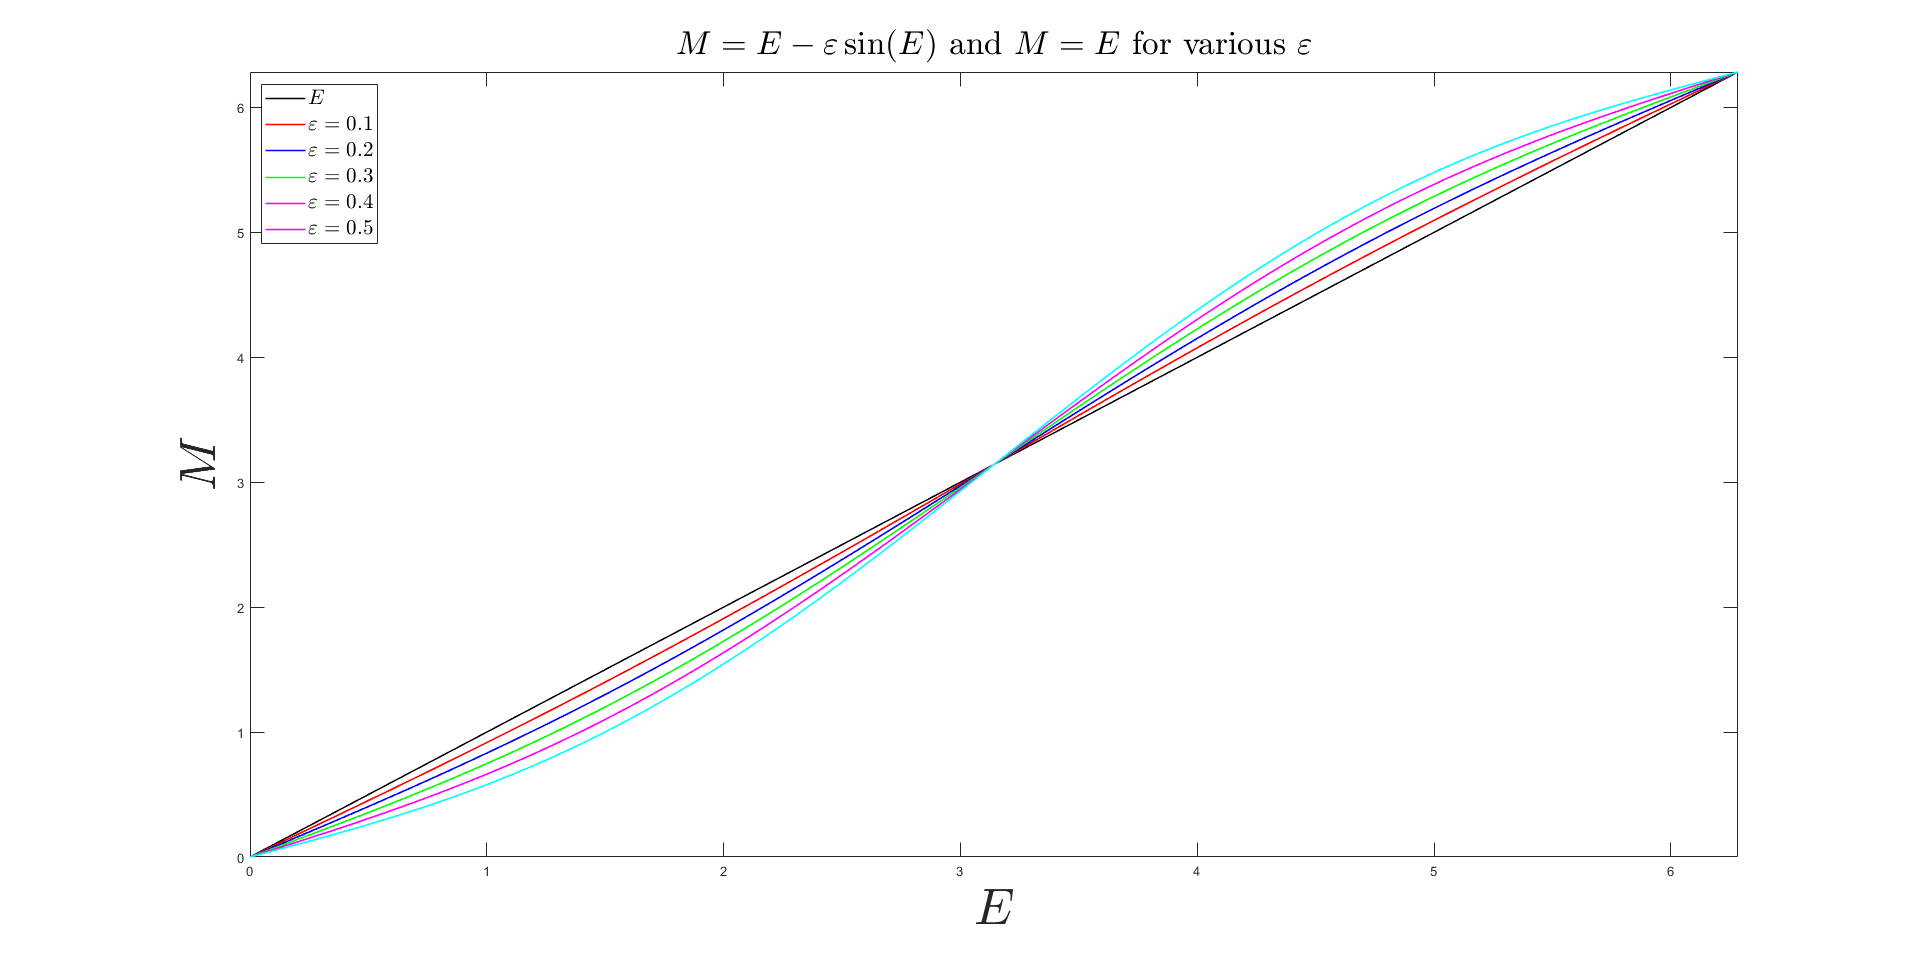
\includegraphics[scale = 0.25]{kepler_eqns.png}
        \end{center}
        From the form of Kepler's Equation, we see that one equation is a $\sin(\cdot)$ function, and one is linear, and since $\sin(x)$ is defined for all $x \in \mathbb{R}$ and bounded between $\pm 1$, and a linear function is bijective on $\mathbb{R}$, we have that there exists at least one equation to Kepler's Equation.
        \newline\newline
        Now, for notational simplicity, define $y = x - \varepsilon\sin(x)$ with $0 \leq \varepsilon < 1$. Here, we identify $x = E$ and $y = M$. We now show that $y$ is monotonically increasing for all $x \in \mathbb{R}$. Notice
        \begin{align*}
            \frac{dy}{dx} &= 1 - \varepsilon\cos(x)\\
            &\geq 1 - \varepsilon > 0
        \end{align*}
        by $0 \leq \varepsilon < 1$. Thus $y$ is monotonically increasing. Now define the ancillary function $f(x) = x - \varepsilon \sin(x) - \tilde{M}$ with $\tilde{M}$ constant. If $\tilde{M} = j\pi $ or $(j+1)\pi$ for $j \in \mathbb{Z}$, we have $f(j\pi) = f((j+1)\pi) = 0$. If $j\pi < \tilde{M} < (j+1)\pi$, then notice 
        \[f(j\pi) = j\pi - \tilde{M} < 0\]
        and 
        \[f((j+1)\pi) = (j+1)\pi - \tilde{M} > 0.\]
        Then by the Intermediate Value Theorem and monotonicity of $f$, we have that $f$ has exactly one root satisfying $j\pi \leq x \leq (j+1)\pi$ whenever $j\pi \leq \tilde{M} \leq (j+1)\pi$. From this analysis, we have that If $M$ satisfies $j\pi \leq M \leq (j+1)\pi$, there is exactly one solution satisfying $j\pi \leq E \leq (j+1)\pi$, as desired.
        \newline\newline

        \item[(b)] The eccentricity for most of the planets in the Solar System is small (e.g., for the Earth $\varepsilon =  0.02$). Assuming $\varepsilon \ll 1$, find the first three terms in an asymptotic expansion for $E$.
        \newline\newline
        \textit{Soln.} From the Taylor expansion for $\sin(E)$, we have
        \[\sin(E) = E - \frac{E^3}{3!} + \frac{E^5}{5!} - \cdots.\]
        Now assume $E \sim E_0 + \varepsilon^{\alpha}E_1 + \varepsilon^{2\alpha}E_2 + \cdots$. From the expansion of $\sin(E)$ and the expansion of $E$, we find
        \begin{align*}
            \sin(E) &= E_0 - \frac{E_0^3}{3!} + \frac{E_0^5}{5!} - \cdots + \varepsilon^{\alpha}\left(E_1 - \frac{3}{3!}E_1E_0^2 + \frac{5}{5!}E_1E_0^4 - \cdots\right) + \cdots\\
            &= \sin(E_0) + \varepsilon^{\alpha}E_1\left(1 - \frac{1}{2!}E_0^2 + \frac{1}{4!}E_0^4 + \cdots\right) + \cdots\\
            &= \sin(E_0) + \varepsilon^{\alpha}E_1\cos(E_0) + \cdots.
        \end{align*}
        Putting these expansions into Kepler's equation, we find
        \begin{align*}
            \varepsilon\sin(E_0) + \varepsilon^{\alpha + 1}E_1\cos(E_0) + \cdots &= E_0 + \varepsilon^{\alpha}E_1 + \varepsilon^{2\alpha}E_2 + \cdots - M
        \end{align*}
        The $\mathcal{O}(1)$ terms give $E_0 - M = 0 \implies E_0 = M$. The $\mathcal{O}(\varepsilon)$ terms give $\alpha = 1$ and $\sin(M) = E_1$. The $\mathcal{O}(\varepsilon^2)$ terms give $\sin(M)\cos(M) = E_2 \implies E_2 = \frac{1}{2}\sin(2M)$. Thus our three term expansion for $E$ gives
        \[E \sim M + \varepsilon \sin(M) + \frac{\varepsilon^2}{2}\sin(2M).\]
        \vspace{0.5cm}

        

        \item[(c)] Show that your result agrees, through the third term, with the series solution
        \[E = M + 2\sum_{n = 1}^{\infty} \frac{1}{n}J_n(n\varepsilon)\sin(nM).\]
         It is interesting that Bessel first introduced the functions $J_n(x)$ when solving Kepler's equation. He found that he could solve the problem using a Fourier series, and this led him to an integral representation of $J_n(x)$. This is one of the reasons why these functions were once known as Bessel coefficients.
         \newline\newline
         \textit{Proof:} From the definition of $J_n(n\varepsilon)$, we have
         \[J_n(n\varepsilon) = \sum_{m = 0}^{\infty}\frac{(-1)^m}{m!(m + n)!}\left(\frac{\varepsilon}{2}\right)^{2m + n}\]
         so that
         \begin{align*}
             J_1(\varepsilon) &= \sum_{m = 0}^{\infty}\frac{(-1)^m}{m!(m + 1)!}\left(\frac{\varepsilon}{2}\right)^{2m + 1}\\
             &= \frac{\varepsilon}{2} - \frac{\varepsilon^3}{8} + \cdots
          \end{align*}
          and
          \begin{align*}
              J_2(2\varepsilon) &= \sum_{m = 0}^{\infty}\frac{(-1)^m}{m!(m+2)!}\left(\varepsilon\right)^{2m + 2}\\
              &= \frac{\varepsilon^2}{2} - \frac{\varepsilon^4}{6} + \cdots.
          \end{align*}
          Thus 
          \begin{align*}
              M + 2\sum_{n = 1}^{\infty} \frac{1}{n}J_n(n\varepsilon)\sin(nM) &= M + \left(\varepsilon - \frac{\varepsilon^3}{4} + \cdots\right)\sin(M) + \frac{1}{2}\left(\varepsilon^2 - \frac{\varepsilon^4}{3} + \cdots\right) + \cdots\\
              &\sim M + \varepsilon\sin(M) + \frac{\varepsilon^2}{2}\sin(nM) + \cdots
          \end{align*}
          which agrees with our three term asymptotic expansion, as desired.
    \end{itemize}
\end{itemize}

\end{document}
